\section{引言}
\label{sec:introduction}

%Large Language Models (LLMs)~\cite{chowdhery2023palm, touvron2023llama, jiang2024mixtral} have emerged as a cornerstone of modern artificial intelligence research, showcasing unparalleled capabilities in generating human-like text, understanding complex queries, and facilitating groundbreaking advancements across numerous domains~\cite{zhang2023prompting, zhang2024benchmarking, siriwardhana2023improving}. The significance of LLMs is underscored by their increasing role in a wide array of applications, from enhancing natural language processing tasks~\cite{adiwardana2020towards, see2017get, yang2016review} to driving innovation in generative AI technologies~\cite{siriwardhana2023improving, github_copilot, cursor}.

随着大语言模型（LLMs）~\cite{chowdhery2023palm, touvron2023llama, jiang2024mixtral} 的规模增长，其训练规模也随之扩大。训练规模的上升使得效率提升不再只是值得追求，而是变得至关重要~\cite{jiang2024megascale}。作为一家为数十亿用户构建 AI 产品的公司，我们持续投入在数千张 GPU 上训练拥有数千亿参数的 LLM。因此，即使训练效率只有边际提升，也能显著减少计算资源消耗和训练时间，并直接影响开发最先进 LLM 的可行性和可持续性。

在 LLM 架构中，专家混合（MoE）模型因稀疏激活而突出~\cite{chowdhery2023palm, jiang2024mixtral, fedus2022switch, shazeer2017outrageously}：它不会让输入 token 经过所有参数，而是将其动态路由到一组被选中的专门网络组件，即 \emph{专家}。随着模型规模增大，这种设计使所需 FLOPs 呈次线性增长，从而显著降低计算成本。
近期工业界进展~\cite{google_GLaM, rajbhandari2022deepspeed, dbrx, grok, liu2024deepseekv3} 展示了 MoE 模型的潜力：在达到相当模型质量的情况下，相比稠密模型可将训练成本降低一个数量级。

尽管 MoE 模型训练成本更低，但从系统角度看，我们观察到训练中的关键性能瓶颈是通信。
例如，在 NVIDIA Hopper GPU 上训练一个内部模型时，通信占前向传播总时间的 43.6\%，并占整个训练过程的 32\%。
这一瓶颈主要来自两个因素。第一，MoE 模型天然引入更多通信开销。相比稠密模型训练，MoE 模型由于参数规模更大，需要分布到更多 GPU 上进行模型并行。第二，为了支持稀疏计算，前向和反向传播中都需要额外两次 all-to-all 通信，分别用于分发和聚合 token，这会阻碍正在进行的计算。

此外，随着硬件进步，计算与通信之间的不平衡越来越明显，通信开销变得更加主导。伴随模型架构改进，硬件能力也快速演进，GPU 处理速度显著提高（图~\ref{fig:gpu_evolution}）。与此同时，训练精度降低也被用于提升训练效率和成本效益~\cite{peng2023fp8, liu2024deepseekv3}。这些趋势共同导致原始计算时间下降，使通信开销的相对影响成为更关键的瓶颈。例如，我们观察到，在某些情况下，仅将现有张量并行扩展到多节点设置就会使通信开销超过 50\%。因此，优化通信对于维持并提升 MoE 模型训练的可扩展性至关重要，尤其是在需要跨多张 GPU 频繁进行数据同步的分布式环境中。

\begin{figure}[t!]
    \centering
    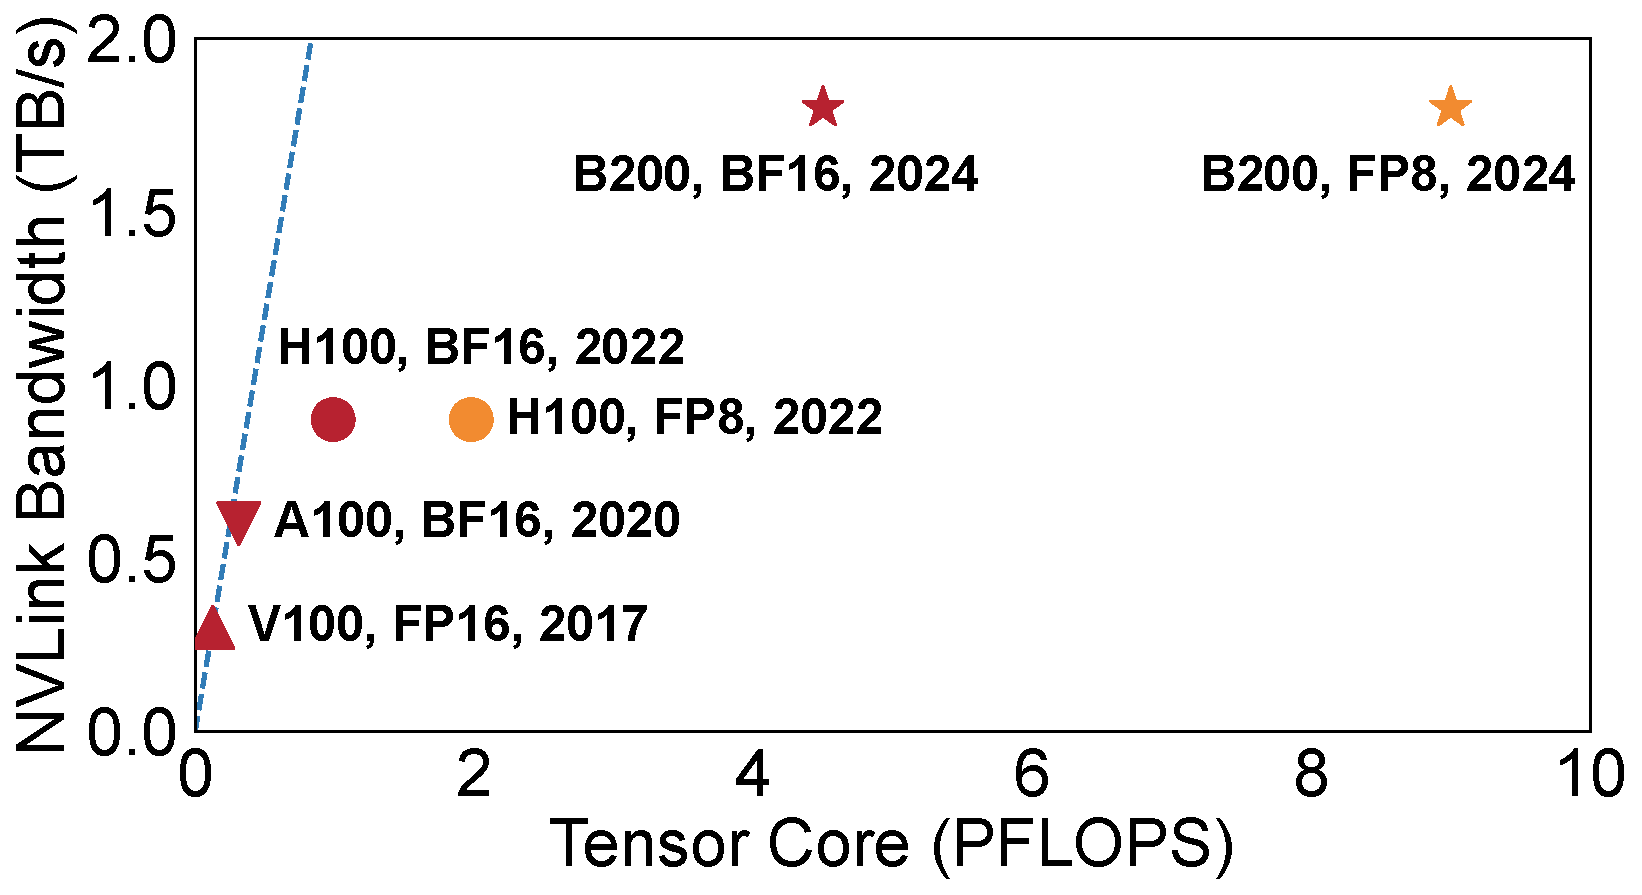
\includegraphics[width=0.75\linewidth]{figures/gpu_evolution.pdf}
    \vspace{-0.1in}
    \caption{NVIDIA GPU 的演进。}
    \vspace{-0.2in}
    \label{fig:gpu_evolution}
\end{figure}

本文介绍 \sysname 的设计、实现和运维经验。它是一个面向高效大规模 MoE 训练优化的生产系统。通过细致处理通信瓶颈，\sysname 试图推进 MoE 训练的边界，并在性能和效率上取得显著提升。
\revision{我们的洞察是：MoE 与稠密模型之间最关键的架构差异位于层内，而这正是通信开销的主要来源。基于这一点，\sysname 将每个 MoE 层限制在单节点内，利用高带宽 NVLink。我们的分析（\S\ref{sec:design:parallelism}）和评估（\S\ref{sec:evaluation}）表明，尽管现有系统~\cite{liu2024deepseekv3, hwang2023tutel} 常采用跨节点专家并行，我们的方法仍能将 MoE 训练有效扩展到数千张 GPU 上的数千亿参数模型。}

具体而言，\sysname 从三个关键方面处理 MoE 训练中的通信问题。第一，\sysname 为每个 MoE 层中的注意力模块和 FFN 模块定制并行策略，以减少通信量。我们比较现有 LLM 训练框架中的并行策略，并全面考虑它们对大规模训练的影响，包括通信量，以及通信能否被有效重叠（即是否位于关键路径上）。
% and their effect on training stability. 
基于这一分析，我们为 MoE 训练选择最优的并行策略组合。

第二，\sysname 在算子层面充分重叠通信与计算。\sysname 将每个 MoE 层的前向和反向传播划分为不同的计算算子与通信算子。对于算子间重叠，\sysname 采用整体化调度策略，在前向和反向传播中精心重排通信和计算算子，将通信隐藏在独立计算之中。该方法还优化了 GPU 内存使用。\sysname 使用选择性激活重物化，在前向传播中仅将部分激活保留在 GPU 内存中，并在反向传播中通过重算或重新通信获得所需激活。借助这种整体化调度，\sysname 有效隐藏重物化开销，在只存储一半激活的同时实现相近性能。

为了重叠关键路径上的通信，\sysname 采用细粒度方法，将通信拆成 tile，并与 GPU 计算模式对齐，把这些 tile 级通信融合进计算 kernel。对于带有 token 分发的 MoE 模型，\sysname 将高效的本地 scatter 操作融合进 kernel，并沿 scatter 后的维度重组计算任务，以缓解来自多个数据源的通信瓶颈。这种细粒度重叠发生在每个节点内部，利用 GPU 之间的高带宽连接。

第三，\sysname 利用通信压缩进一步提升 MoE 训练效率。具体而言，对于广泛使用的 BF16 混合精度训练，\sysname 将跨节点参数同步精度从 FP32 降到 BF16，使相关开销减半。在 FP8 训练中，\sysname 用 FP8 通信替代 BF16 reduce-scatter，并结合定制量化策略和 FP32 归约，在保持收敛稳定性的同时降低通信量。

\sysname 已部署在我们的数据中心，用于为产品训练 MoE 模型。相比最先进的开源 LLM 训练框架 Megatron-LM~\cite{shoeybi2019megatron}，在 1,440 张 NVIDIA Hopper GPU 上训练 352B MoE 模型时，\sysname 的 MFU（Model FLOPs Utilization）最高提升 1.88$\times$。凭借全面的通信优化，\sysname 支撑了我们生产环境中的大规模训练，高效扩展到万亿参数和数千张 GPU，并节省了数百万 GPU 小时。
